\documentclass[9pt]{article}
\pagestyle{empty}
\usepackage{fancyhdr}
\usepackage{lastpage}
\usepackage{graphicx}
\graphicspath{ {images/} }
\pagestyle{fancy}
\renewcommand{\headrulewidth}{0pt}
\cfoot[R]{\thepage~of~\pageref{LastPage}}
\addtolength{\oddsidemargin}{-.875in}
\addtolength{\evensidemargin}{-.875in}
\addtolength{\textwidth}{1.75in}
\addtolength{\topmargin}{-.875in}
\addtolength{\textheight}{1.75in}

\begin{document}
\begin{center}
\textbf{Database Systems Homework 1}
\end{center}

\\ We are required to produce an ER diagram from the following:
\begin{enumerate}
    \item There is an entity set Person. It has attributes L-number which identifies a person entity, email and Name. The value of L-number and Name are always known. No two persons can have the same value of L-number.
    \item There is an entity set, Librarian, which is a set of some of the entities in Person. It has attributes Salary and SSN with the latter always known.
    \item There is an entity set, Patron, which is a set of some of the entities in Person. It has an attribute Fine and a composite attribute ID, which consists of attributes Type (e.g., Driver’s license) and Value (e.g., License number), which are always known. No two patrons can have the same values of both Type and Value
    \item An entity in Person is in at least one of the entity sets Librarian and Patron.
    \item There is a binary relationship Supervises between Librarian and itself. We assign the roles of Supervisor and Supervisee to a pair of entities in Librarian participating in Supervises. Every Supervisee can have at most one Supervisor. The relationship Supervises has an attribute Date which represents the date on which the Supervisee was assigned to the Supervisor.
    \item There is a binary relationship Advises between Librarian and Patron. This relationship shows that patrons are advised by some librarians. It has an attribute Date which represents the latest date on which the librarian advised the patron. It’s value is always known.
    \item There is an entity set Book. It has attributes Author, ISBN and Title. The values of these attributes are always known. An entity in Book can be identified by specifying ISBN. Author can have any number of values.
    \item There is an entity set Publisher. It has an attribute Name, which identifies an entity in Publisher and another attribute Editor.
    \item There is an entity set City. It has attributes State, Name and Size. A city can be identified by specifying both State and Name, but not by only one of them.
    \item There is a ternary relationship Publishes among Book, Publisher, and City. The relationship has an attribute Year, the value of which is always known. A book is published by exactly one publisher and in exactly one city.
    \item There is an entity set Copy. It has an attribute Number.
    \item Each book in the library is stored as one or more physical copies, and physical copies of the same “abstract” book have different copy numbers. There is a binary relationship Stored between Book and Copy which states what are the copies of the books that are stored. For example a particular ISBN can be stored as copies 1, 2, 4, and presumably copy 3 was lost.
    \item There is a binary relationship Borrows between Patron and Copy. It has attributes Due, which is the due date for the borrowed book, whose value is always known. There is also an attribute Fine. If the current date is later than the due date, then the value of Fine is the number of days past due multiplied by \$2, otherwise it is empty. Also, a patron can borrow at most 20 physical copies.
    \item The attribute Fine of a Patron is the sum of all the fines on the books the patrons has borrowed.
\end{enumerate}
The ER diagram was created using Microsoft Visio 2010.
\begin{center}
    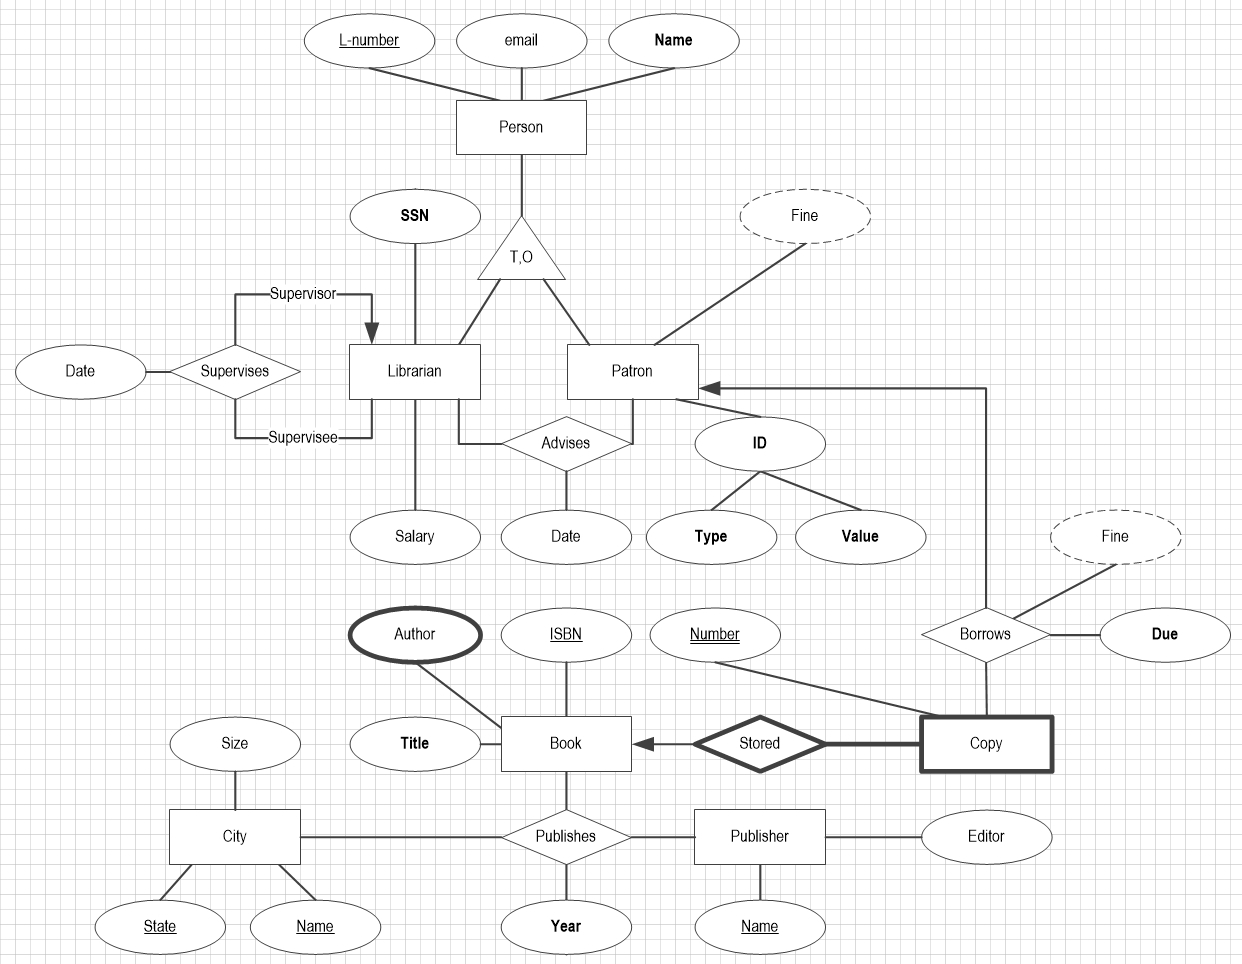
\includegraphics[width=180mm]{solution.jpg}
\end{center}
The ER diagram has the following annotations on a second page:
\begin{itemize}
    \item A \textbf{Patron} can borrow at most 20 books
    \item For a \textbf{Librarian}, \textbf{SSN} is never Null
    \item For a \textbf{Patron}, \textbf{Type} and \textbf{Value} are never Null and no two patrons can have the same tuple (\textbf{Type}, \textbf{Value})
    \item \textbf{SSN} in \textbf{Librarian} is never Null, \textbf{Date} in \textbf{Advises} is never Null, \textbf{Due} in \textbf{Borrows} is never Null, \textbf{Title} in \textbf{Book} is never Null
    \item \textbf{Fine} in \textbf{Borrows} is calculated if the book is overdue i.e. if Current Date $<$ Due Date then \textbf{Fine} = (Due Date - Current Date)*2, otherwise it is Null
    \item \textbf{Fine} in \textbf{Patron} is the sum of the fines on books patron has borrowed and not yet returned
    \item Each \textbf{Book} is published by a single \textbf{Publisher} and in a single \textbf{City}
\end{itemize}

\end{document}